% -*-mode: Latex-*-
% !TEX root = thesis.tex
% paper: ...
% authors: simon maurer
%
% file: introduction.tex
% contents: introduction to the thesis
% Sccs-Id: %W% %G%
\chapter{Introduction}
\label{chap_intro}
Nowadays, with microcontrollers getting smaller and more efficient, computing is becoming more and more pervasive in our everyday life.
This is achieved by embedding computer devices in physical objects such that the computing devices interact with the physical world.
Such systems are called \glspl{cps}.
A \gls{cps} is a reactive system that senses its environment (the physical world), performs a computation on a computational entity (this can be anything from a simple embedded device to a large scale distributed system), and then actuates on the environment according to the computations.
The actuation on the environment causes the environment to change which, in turn, is detected by the sensors and the computation is performed with the new dataset.
Typically, this reactive loop is time-critical and is executed as long as the system is running.
In contrast to a traditional embedded system, \ie a time-critical system, dedicated to a single hardware platform, a \gls{cps} tends to be an assembly of networked subsystems where some subsystems interact with the physical world and some may be purely computational.

Examples of \glspl{cps} can be found in the domain of automotive vehicles (\eg anti-lock braking system, adaptive cruise control, electronic stability control, platooning), avionic vehicles (\eg flight control systems, black box, pressure control), or smart spaces (\eg intelligent highway control, building control), to name only a few.

Because of the direct interaction of \glspl{cps} with the physical world, it is often crucial to respect timing requirements imposed by the physical world to guarantee a correct behaviour of the system.
In case of critical applications such as nuclear power plants, avionic systems, or cars, huge efforts are made to verify the correct behaviour of the application.
The main difference between critical systems and best-effort systems is that critical systems are designed for the worst case whereas best-effort systems are designed for the average case.
Henzinger and Sifakis argue that over time, this difference led to a gap between the models employed in the two domains and that the gap is continuing to widen~\cite{henzinger2006}.
Due to the difference of the employed models, critical and non-critical applications tend to be physically separated and run on dedicated hardware platforms.
This is a problem because with the evolution of hardware towards multi/many-core architectures, there is the interest to integrate components with different criticality requirements on the same platform.
Such systems are typically called mixed-criticality systems~\cite{burns2016}.
What adds further to the challenge of integrating \glspl{cps} on a multi/many-core architecture is that \glspl{cps} are often heterogeneous in the sense that several applications from different domains with different characteristics must coexist or interact with each other~\cite{eker2003}.
Eker \etal address this challenge by assembling multiple models, each suitable for its specific application domain, in one framework~\cite{eker2003}.
Others argue that one meta model, allowing to describe and compose heterogeneous systems, is more beneficial because it provides a better ground for a meaningful analysis of the system~\cite{henzinger2006, rajkumar2010, castrillon2015}.
% This is also referred to as model-based design.

Another challenge is the inherent concurrency of \glspl{cps}~\cite{lee2008}.
Streaming networks are well-recognised for coping with concurrent systems~\cite{stephens1997}.
They consist of processing nodes (often called filters) connected via communication channels where a channel is connected to a single producer node and a single consumer node.
This property of streaming networks, combined with the implicit synchronisation of producers and consumers due to a blocking channel access, allows to tame the complexity of concurrent systems which makes them also an interesting paradigm to apply to \glspl{cps}.
However, current streaming models (\eg~\cite{thies2002, lee2003, grelck2010}) tend to rely on the possibility that a system can be decomposed into transformational components such that the behaviour of a component can be described as a pure function.
Such a decomposition makes it easier to understand component dependencies and allows to analyse the system, \eg for schedulability~\cite{lee1987} or deadlocks~\cite{zhou2006}.
However, given that \glspl{cps} are often systems of reactive nature, such a decomposition is difficult~\cite{harel1985}.

An interesting approach where no decomposition in transformational components is required are interface theories~\cite{deAlfaro2001} which allow to describe components with arbitrary behaviour by their interfaces and build complex components out of simple ones by composition.
Several interface models have been proposed to describe communication compatibility between components~\cite{deAlfaro2001a, larsen2006, hennicker2015} as well as additional properties such as modalities~\cite{larsen2007}, resource usage~\cite{chakrabarti2003, thiele2006}, or timing constraints~\cite{dealfaro2002, henzinger2006a}.
However, these models do not target streaming networks and lack the capability of describing the blocking semantics of message passing in streaming networks.

In this dissertation I introduce a novel automata-based interface description model, called \gls{sia}, that allows to describe the interaction protocol of processes with their environment.
\Glspl{sia} are suitable to describe the blocking semantics of \gls{kpn}-based~\cite{kahn1974} streaming networks and thus serve as a powerful tool to bridge the gap between \gls{lts} and stream processing.
An incremental composition operation allows to build complex processes out of simple ones.
A novelty of the \gls{sia} model is that it allows to identify permanent blocking situations (\eg deadlocks) in a composed network due to the blocking semantics of the model.
The inspiration for the \gls{sia} model stems from \glspl{ia}~\cite{deAlfaro2001a}.
The blocking semantics of the here presented \glspl{sia} differs fundamentally from the blocking semantics of \glspl{ia}.
This enables \glspl{sia} to describe process networks where processes interact with synchronous communication, \eg~stream processing applications.

I further introduce a novel component-based model, called \gls{pnsc} that serves as a wrapper for \glspl{sia} and allows to model an assembly of reactive processes, \ie processes capable of consuming and producing streams of infinite length.
I extend the model to support the coexistence and interaction of processes with an event-triggered and a time-triggered execution scheme.
In the former case, sporadically occurring events are causing a subsystem to perform its computation while in the latter case a fixed schedule imposes time instances when a subsystem is performing its computation.
There are application domains where both models are required (\eg automotive domain) but the two models are often used in limited ways to just co-exist but do not directly interact with each other (\eg~\cite{ferreira2002, steiner2011, obermaisser2006}).
The problem is that interaction may cause interference from a subsystem of low criticality towards a subsystem of high criticality which must be avoided.
A novelty of the extended \gls{pnsc} model is that it allows not only the co-existence of the two triggering semantics in the same system but also allows interaction between time-triggered subsystems and event-triggered subsystems.
The key point is to guarantee that the event-triggered subsystem, having a lower criticality level, is not interfering with the time-triggered subsystem of higher criticality.
Further, the model allows to use the same mechanism to avoid interference from a lower critical event-triggered subsystem to a higher critical event-triggered subsystem.
Two time-triggered subsystems do not interfere with each other out of construction~\cite{kopetz2002}, independent of their criticality level.

To provide control on communication bandwidth usage, the model allows to limit the communication rate of a process to an upper bound.
This is achieved with a novel approach of controlling message passing between processes with different consequences depending on the message semantics.

A challenge related to the inherent concurrency of \glspl{cps} is the efficient execution of concurrent systems on multi-core hardware platforms.
With the ever growing capabilities of integrated circuits due to the persistence of Moore's law, software engineers face the challenge to design, develop, and maintain complex software systems that exploit the available computation power.
As a consequence of reaching the power wall through frequency scaling~\cite{pollack1999}, parallel hardware architectures have been designed.
Even in the domain of embarrassingly parallelisable applications where it is easy to split the computation load in a large number of independent computational chunks due to lack of data or code dependencies, parallelization remains not a simple task because of the tight coupling between hardware and software (\eg efficient use of memory hierarchy) and the inherent difficulty of debugging parallel code.
Nowadays, there are tools, libraries, and languages available that help to cope with some of the problems.
In the domain of Big Data on large scale distributed systems examples are Hadoop\footnote{\url{http://hadoop.apache.org/}}, HPCC\footnote{\url{https://hpccsystems.com/}}, and Hydra\footnote{\url{https://github.com/addthis/hydra}}.
For shared memory multi-core architectures some examples are Cuda\footnote{\url{http://www.nvidia.com/object/cuda_home_new.html}}, OpenMP\footnote{\url{http://www.openmp.org/}}, and TBB\footnote{\url{https://www.threadingbuildingblocks.org/}}.

However, multi- and many-core processor architectures have emerged to a broad variety of application fields, including \glspl{cps}, where it is hard to identify potential blocks that can exhibit parallelism due to dependencies between tasks and, especially, due to the reactive nature of \glspl{cps}.
In their survey on programming solutions for multicore architectures in the domain of \glspl{cps}, Castrillon \etal note that even though achievements were made in academia, in industry, \gls{cps} software development for parallel architectures remains mostly manual~\cite{castrillon2015}.
A reason for this is that industry often relies on legacy code that may include system libraries or multiple layers of mixed languages which is often ignored by academic solutions (\eg introducing a new language requires industry to rewrite lots of legacy source code in the new language which they may be hesitant to do).

To cope with concurrency in applications, programming languages either incorporate models (\eg Actor model~\cite{agha1985} in Scala, \gls{csp}~\cite{hoare1978} in Ada) or libraries are provided (Open \gls{mpi}~\cite{open-mpi}) to simplify design, development, and maintainability of the application.
While such models certainly help to structure the code and enforce good practices in parallel programming, it is still up to the programmer to separate between coordinational and computational aspects of the program.
While an expert in a certain application domain - a \emph{domain expert} - is very adept in solving problems and working with models related to this domain, it is rarely his or her expertise to cope with the inherent problems of concurrency and parallelization.

An interesting approach to solve this problem is to separate the different concerns of an application, as proposed by Gelernter and Carriero in~\cite{gelernter1992}.
The main idea is to separate the concerns of computation and coordination by using a coordination language in addition to a programming language.
This allows the domain expert to choose a language that suits his needs to program computational blocks which are then linked together, potentially by another person, using a coordination language based on a model that is suitable to cope with concurrency.
This clear separation of concerns is an intriguing concept, especially for interdisciplinary application fields where experts from different domains work together.
As \glspl{cps} tend to describe applications in interdisciplinary fields, a clear separation of concerns is desirable.

In this dissertation I introduce a new coordination language, called \gls*{smx}, that is based on the \gls{pnsc} model, also introduced in this thesis.
While \gls*{smx} is an instantiation of the \gls{pnsc} model, the language provides more than just concrete syntax for the model:
\Gls*{smx} allows to describe a network of processes in a structured and hierarchical manner due to its usage of network composition operators.
This is inspired by the coordination language \gls*{snet}~\cite{grelck2010} which allows to describe networks of pure components.
The novelty of \gls*{smx} is that while it is based on the stream processing paradigm it retains the capability of describing \glspl{cps} where components are hard to decompose due to the reactive nature of \gls{cps}.
\Gls*{smx} is an exogenous coordination language where the coordinated components are unaware of the coordination exert on them~\cite{arbab2006}.

This dissertation describes a holistic approach, reaching from the underlying theory of the coordination model to an instantiation of the model in the form of a language and a prototype toolchain that allows to compile \gls*{smx} code into an executable C program, check the program for permanent blocking, and link it with C implementations of \gls{pnsc} processes.
The resulting application can be executed on a platform with support for ISO C, POSIX threads, and a Linux operating system.


%==============================================================================
\section{Thesis and Research Questions}
\label{sect_intro_question}
In this section I present the thesis this dissertation aims to maintain and several research questions that guided me through my research.
As described in the beginning of this chapter, my work aims at using models from different fields, namely stream processing and interface theory, and adapt the models in such a way that they are applicable for \glspl{cps}.
Consequently, I formulate my thesis as follows:
\begin{center}
    \rule[5mm]{\textwidth}{0.4pt}
    \parbox{0.8\textwidth}{
    \centering
        \emph{It is possible to bridge the gap between stream processing and \acrfullpl{lts} for complex components.}
    }
    \rule[-2mm]{\textwidth}{0.4pt}
\end{center}

In the following I will describe several research questions that focus on sub-aspects of the thesis and help to dissect each aspect independently.
I first ask a general question about coordination models to then refine it with three more precise questions:

\paragraph*{How to coordinate mixed-criticality CPSs?} \hfill

To answer this question, as a first step, it is crucial to identify properties of \glspl{cps} and understand how they relate to coordination aspects.
A mixed-criticality \gls{cps} is an assembly of networked subsystems with strong and weak coupling between them.
Some of the subsystems are critical systems, \ie of high criticality, some are best-effort systems, \ie of low criticality.
The coupling between the different subsystems is of various degrees.
Critical subsystems tend to have a weak coupling with other subsystems to prevent mutual interference while best-effort systems tend to be strongly coupled.
A coordination model for a mixed-criticality \gls{cps} must be able to model these various degrees of coupling between subsystems while providing guarantees of correctness of the overall behaviour of the system.

To refine the research question I ask two follow-up questions centring around the coupling of subsystems.
A third follow-up question focuses on coordination languages and the implication of reactive components on a language.

\paragraph*{What are suitable interfaces for reactive components with strong coupling to ensure correct behaviour of a system of such components assembled in a network?} \hfill

A main property of a component that supports reactive behaviour is that it must be able to cope with infinite streams, \ie potentially run infinitely.
Due to this property, a component must support to read an input as a reaction to writing an output.
This is because of a potential coupling between the output and the input through the environment.
This must be reflected in the interface describing the component.
In this dissertation I introduce the automata-based model \gls{sia} that allows to describe the interaction of a component with its environment.
\Glspl{sia} are based on a strict blocking semantics, modelling synchronous communication, which allows to describe streaming applications and their inherent strong coupling between components.
The \gls{sia} model allows the composition of simple components into more complex ones while preserving the blocking semantics.
I further introduce an analytic method, based on the \gls{sia} model, to detect situations where components are blocking indefinitely, \eg deadlock situations.

% A related but more general topic is discussed by Henzinger and Sifakis~\cite{henzinger2006}.
% They observed that the gap between engineering methodologies for critical systems and best-effort systems is widening.
% As a solution to bridge this gap, they proposed to unify heterogeneous systems under one meta-model that allows the composition of components while preserving properties.
% This same principle holds for coordination models for \glspl{cps} where the focus lies on communication and synchronisation.

% \emph{What are suitable coordination elements to support time-criticality in \glspl{cps}?}

% Guarantees on timing requirements create a tight bound between hardware and software and require a system to be predictable and analysable.
% Interfaces have to be provided that allow to perform model checking and verification processes on the subcomponents of the system.
% In addition, the model needs to provide facilities to annotate individual subcomponents with timing requirements.\\

\paragraph*{What are suitable interfaces for CPSs to integrate subsystems with different criticality levels?} \hfill

In contrast to a strong coupling, addressed in the previous question, a weak coupling allows to ensure the system correctness based on the component correctness.
The focus of this question lies on the interaction of subsystems with different degrees of coupling.
A main challenge of a mixed-criticality system is to allow multiple subsystems with different criticality levels to co-exist on the same platform or even to interact with each other.
The challenge of such a configuration is to assure that the subsystems with lower criticality levels do not interfere with subsystems of higher criticality levels.
In this dissertation I introduce \glspl{cci} that allow to selectively implement a weak coupling between two components and prevent such an interference.

\paragraph*{What are the implications of reactive components on an exogenous coordination language?} \hfill

The interaction of subsystems in a \gls{cps} is often based on reactive data processing where the environment imposes a link between the inputs and outputs of the component.
A reactive component is hard to decompose because reactive components tend to rely on persistent state and internal synchronisation points.
Due to this, simple and intuitive language primitives are required to describe reactive communication patterns in a structured way, such as chained components with mutual bi-directional interaction, without loosing in terms of locality.
I adopt the notion of network operators to describe a network of reactive components.
Different types of operators allow to describe a network in a structured and hierarchical manner by keeping information local.


%==============================================================================
\section{Contributions}
\label{sect_intro_contribution}

To illustrate the contribution of this dissertation, \Fig{\ref{fig_trinity}} provides a simplistic overview of related work and the gap between research fields that this dissertation aims to bridge.
In the figure, three circles represent three aspects that tend to be part of a \gls{cps}.
Each circle is associated with a model that allows to describe particular properties of each aspect and tackle the challenge they pose for modelling \glspl{cps}.
\begin{itemize}
    \item \Glspl{cps} tend to be \emph{concurrent} due to the fact that they interact with the physical world which is inherently concurrent~\cite{lee2008}.
        In this work, concurrency aspects are tackled with a stream processing model which provides inherent synchronisation between interacting components.
    \item \Glspl{cps} tend to be \emph{heterogeneous} with respect to multiple aspects such as mixed-criticality~\cite{burns2016}, different timing
        semantics~\cite{kopetz2011}, or different underlying theoretical models~\cite{eker2003}.
        In this dissertation I focus on mixed-criticality aspects and different timing semantics and use well defined communication interfaces, called \glspl{cci}, to control the interaction between components.
    \item \Glspl{cps} tend to be \emph{reactive} systems with complex interacting components which are hard to decompose~\cite{harel1985}.
        In order to support complex components in a stream processing model I introduce the novel \gls{sia} model, an analysable component abstraction.
\end{itemize}

Further, the figure shows a few examples of related work, prominent representatives of their domain, that are placed in the circles or the intersection of two circles to illustrate which aspects of \glspl{cps} are covered by their respective model.
The symbolic dial, surrounding the three circles, represents the time-criticality aspect of \glspl{cps}.
Of the represented models only the names that are not greyed-out support some sort of control over timing behaviour.
The figure illustrates a clear gap between reactive systems with support for complex components and stream processing models.
This gap is filled by the work presented in this dissertation, namely the \gls{pnsc} model and the extension of the model.

%------------------------------------------------------------------
\begin{figure}[bht]
    \TopFigSpace
    \vspace{2mm}
    \centering
    \includegraphics[width=10cm]{fig/trinity.pdf}
    \CaptionFigSpace
    \vspace{2mm}
    \caption{A simple schematic representation of properties of \glspl{cps} and how the novel \gls{pnsc} model bridges the gap between stream processing and \gls{lts} for complex componets.}
    \label{fig_trinity}
    \BotFigSpace
\end{figure}
%------------------------------------------------------------------

The work described in this dissertation provides the following novelties and contributions:
\begin{itemize}
    \item introduction of a novel exogenous, component-based coordination model, called \gls{pnsc}, that allows to describe networks of processes, communicating through sporadic message passing.
        The novelty of the model is an \gls{lts}, called \gls{sia}, first introduced in this dissertation, that allows to capture the blocking semantics of interacting processes.
        The model allows to describe processes with persistent state and internal synchronisation points.
        These are properties that fit well with the requirements of \glspl{cps} which tend to be networks of reactive components.
        A composition operator allows to compose processes while preserving the properties of blocking communication.
    \item extension of the novel \gls{pnsc} model.
        The extensions have no influence on the behavioural aspect of a process which preserves the exogenous coordination property of the \gls{pnsc} model.
        The extensions provide support for
        \begin{itemize}
            \item mixed-criticality systems through selective communication decoupling to prevent unwanted interference between processes.
                The extension integrates seamlessly with \glspl{sia} which are used to describe the communication decoupling mechanism.
            \item multiple process execution schemes in a process network.
                This is achieved by using the communication decoupling mechanism in conjunction with clock signals to enforce a time-triggered process execution on a subset of processes.
                The model allows to enforce time-triggered communication on individual processes or on a network of processes.
            \item rate-controlled event-triggered communication.
                This is also achieved through selective communication decoupling.
                Two types of protocols are proposed, each applicable in a buffered and non-buffered situation, to enforce a limit on the communication rate.
        \end{itemize}
    \item proposition of the novel message type \emph{semi-state} which complements the well known message semantics of state messages and event messages in the context of stream processing.
    \item development of a novel static analysis, based on the interface theory with \gls{sia}, that allows to detect permanent blocking situations in the network.
        The analysis distinguishes between deadlock and lonely blocking situations.
    \item introduction of the novel exogenous coordination language \gls*{smx}.
        \Gls*{smx} is an instantiation of the \gls{pnsc} model.
        It allows to describe a network of complex reactive processes in a structured and hierarchical manner.
    \item development of a toolchain including a \gls{rts}, compiler, and permanent blocking checker that allows to produce executable applications by describing a system network by a \gls*{smx} program and linking it to individual C implementations and \gls{sia} descriptions of \gls{pnsc} processes.
        The resulting application can be executed on a platform with support for ISO C, POSIX threads, and a Linux operating system.
\end{itemize}

%------------------------------------------------------------------------------
\subsection{Publications}
The following conference and workshop publications resulted from my research and have been published:
\begin{itemize}
    \item \bibentry{maurer2015}
    \item \bibentry{maurer2015a}
    \item \bibentry{kirner2015}
\end{itemize}
The following journal publication is ready for submission:
\begin{itemize}
    \item \bibentry{maurer2017}
\end{itemize}

%==============================================================================
\section{Structure of this Dissertation}
\label{sect_intro_structure}
The remainder of this dissertation is structured as follows:
\begin{description}
    \item[\Chap{\ref{chap_background}}] provides background information on concepts I use throughout the dissertation and discusses terminology.
        The related topics are component-based design and more specifically interface theory, \glspl{cps} and their challenges, different communication models in \glspl{cps}, and coordination languages.
    \item[\Chap{\ref{chap_ecm}}] introduces the \gls{pnsc} model that allows to describe networks of processes.
        The interaction of a process with its environment follows a clearly defined blocking semantics.
        In this chapter I further introduce the automata-based \gls{sia} model that allows to describe the interaction protocol of a process as its interface with its environment and I define a composition operator that allows to compose \gls{pnsc} processes in arbitrary order.
    \item[\Chap{\ref{chap_tcm}}] describes an extension to the \gls{pnsc} model that allows to punctually loosen the communication coupling between interacting processes.
        This can be used to model mixed-criticality systems, based on a sporadic communication scheme to prevent undesired interference.
        The chapter further describes that, in conjunction with clock signals, the decoupling elements allow to construct temporal firewalls which can be used to change the sporadic communication model of a subset of processes to a time-triggered communication model.
        In this chapter I further introduce rate-control mechanisms to bound communication rates of processes to a maximum limit.
    \item[\Chap{\ref{chap_block}}] introduces a permanent blocking analysis that allows to identify permanent blocking situations in a \gls{pnsc}.
        Further, the chapter introduces the distinction between deadlock situations and lonely blocking situations.
    \item[\Chap{\ref{chap_smx}}] describes the coordination language \gls*{smx} which represents an instance of the extended \gls{pnsc} model.
        \Gls*{smx} is an exogenous coordination language that allows to compose reactive components in a structured and hierarchical manner to form a network of processes.
    \item[\Chap{\ref{chap_tool}}] describes a prototype of a toolchain for the coordination language \gls*{smx}.
        It includes the compiler for the \gls*{smx} language, the \gls{rts} preprocessor, the \gls{rts}, and the \gls{sia} model checker.
        Together, the tools allow to build an application that can be executed on a platform with support for ISO C, POSIX threads, and a Linux operating system.
    \item[\Chap{\ref{chap_related}}] compares the different aspects of my work with the state of the art.
        This includes interface theory, mixed-criticality models, coordination languages and models, and methods to detect or prevent permanent blocking situations.
    \item[\Chap{\ref{chap_conclusion}}] finally concludes the dissertation and discusses the results and contributions of the thesis.
        It also includes directions for future research on this topic.
\end{description}

